\documentclass[twoside]{article}


\usepackage[sc]{mathpazo} % Use the Palatino font
\usepackage[T1]{fontenc} % Use 8-bit encoding that has 256 glyphs
\linespread{1.3} % Line spacing - Palatino needs more space between lines
\usepackage{microtype} % Slightly tweak font spacing for aesthetics

\usepackage[hmarginratio=1:1,top=32mm,columnsep=20pt]{geometry} % Document margins
\usepackage{multicol} % Used for the two-column layout of the document
\usepackage[hang, small,labelfont=bf,up,textfont=it,up]{caption} % Custom captions under/above floats in tables or figures
\usepackage{booktabs} % Horizontal rules in tables
\usepackage{float} % Required for tables and figures in the multi-column environment - they need to be placed in specific locations with the [H] (e.g. \begin{table}[H])
\usepackage{hyperref} % For hyperlinks in the PDF

\usepackage{lettrine} % The lettrine is the first enlarged letter at the beginning of the text
\usepackage{paralist} % Used for the compactitem environment which makes bullet points with less space between them

\usepackage{titlesec} % Allows customization of titles
\renewcommand\thesection{\Roman{section}} % Roman numerals for the sections
\renewcommand\thesubsection{\Roman{subsection}} % Roman numerals for subsections
\titleformat{\section}[block]{\large\scshape\centering}{\thesection.}{1em}{} % Change the look of the section titles
\titleformat{\subsection}[block]{\large}{\thesubsection.}{1em}{} % Change the look of the section titles

\usepackage{fancyhdr} % Headers and footers
\pagestyle{fancy} % All pages have headers and footers
\fancyhead{} % Blank out the default header
\fancyfoot{} % Blank out the default footer
\fancyhead[C]{USC EE483} % Custom header text
\fancyfoot[RO,LE]{\thepage} % Custom footer text



\usepackage{multicol}
\usepackage{listings}
\usepackage{graphicx}
\usepackage{caption}
\usepackage{subcaption}
\usepackage{hyperref}
\usepackage{color}
\usepackage{float}
\usepackage{mathtools}
\usepackage{amssymb}
\usepackage{wrapfig}


\lstset{ %
language=Matlab,                % choose the language of the code
basicstyle=\footnotesize,       % the size of the fonts that are used for the code
numbers=left,                   % where to put the line-numbers
numberstyle=\footnotesize,      % the size of the fonts that are used for the line-numbers
stepnumber=1,                   % the step between two line-numbers. If it is 1 each line will be numbered
numbersep=5pt,                  % how far the line-numbers are from the code
backgroundcolor=\color{white},  % choose the background color. You must add \usepackage{color}
showspaces=false,               % show spaces adding particular underscores
showstringspaces=false,         % underline spaces within strings
showtabs=false,                 % show tabs within strings adding particular underscores
frame=single,           % adds a frame around the code
tabsize=2,          % sets default tabsize to 2 spaces
captionpos=b,           % sets the caption-position to bottom
breaklines=true,        % sets automatic line breaking
breakatwhitespace=false,    % sets if automatic breaks should only happen at whitespace
escapeinside={\%*}{*)}          % if you want to add a comment within your code
}
%----------------------------------------------------------------------------------------
%	TITLE SECTION
%----------------------------------------------------------------------------------------
\begin{document}
\thispagestyle{fancy} % All pages have headers and footers
\noindent \textbf {2}
\begin{lstlisting}
% solution2
a = zeros(17,18);
c = 0.4636;
for l = 1 : 17
    a(l,1:2) = [1-c*exp(1j*( (8+l)/17 )*pi),-1-c*exp(1j*( (8+l)/17 )*pi)];
end
multifft = ones(1,18);
for l = 1 : 17
    multifft = fft(a(l,:)) .* multifft; 
end
coefficientDe = ifft(multifft);
% dominator
dominator = zeros(1,18);
for i = 0 : 17
    dominator(i+1) = nchoosek(17,i);
end
dominator = c^17 * dominator;
[h,w]=freqz(dominator,coefficientDe);
plot(w/pi,abs(h));
title('magnitude');
\end{lstlisting}
\begin{multicols}{2}
\begin{figure}[H]
   \centering
   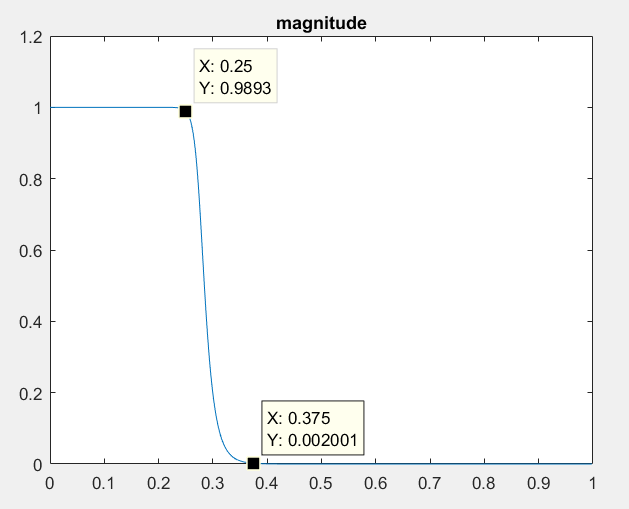
\includegraphics[width = 0.45\textwidth]{./data/solution2.png}  
   \caption{magnitude responce}
\end{figure}
\begin{figure}[H]
   \centering
   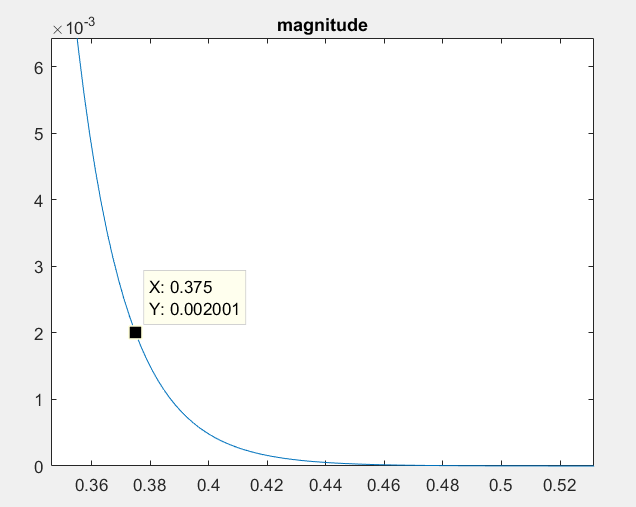
\includegraphics[width = 0.45\textwidth]{./data/solution2error.png}  
   \caption{ripple}
\end{figure}
\end{multicols}

% \noindent \textbf {3}
\noindent \textbf {3(a)}\\
\begin{lstlisting}
b = firpm(14, [0,0.25,0.45,1], [1,1,0,0]);
[h,w]=freqz(b);
plot(w/pi,abs(h));
title('magnitude')

figure
b = firpm(14, [0,0.5,0.6,1], [1,1,0,0]);
[h,w]=freqz(b);
plot(w/pi,abs(h));
title('magnitude')
\end{lstlisting}
\begin{multicols}{2}
\begin{figure}[H]
   \centering
   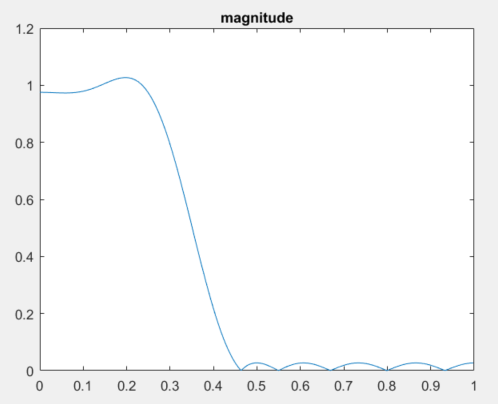
\includegraphics[width = 0.5\textwidth]{./data/solution3a1.png}  
   \caption{$\omega_c = 0.35\pi$}
\end{figure}
\begin{figure}[H]
   \centering
   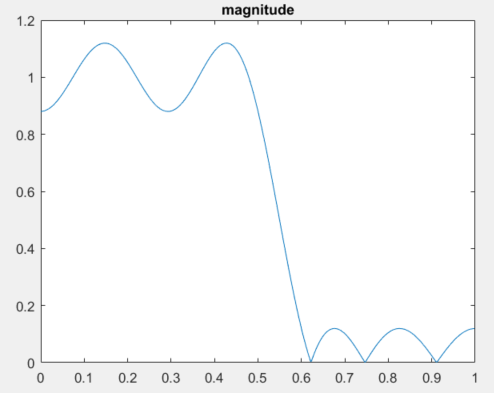
\includegraphics[width = 0.5\textwidth]{./data/solution3a2.png}  
   \caption{$\omega_c = 0.55\pi$}
\end{figure}
\end{multicols}
\noindent \textbf {3(b)}\\
\begin{lstlisting}
b = firpm(14, [0,0.25,0.45,1], [1,1,0,0]);
[h,w]=freqz(b);
plot(w/pi,abs(h));
title('magnitude')


beta = -0.3129;
Mat = zeros(14,15,15);
for i = 1 : 14
    Mat(i,:,1) = [1,-beta,zeros(1,13)];
end
for i = 1 : 14
    Mat(i,:,15) = [-beta,1,zeros(1,13)];
end
for j = 2:13
    for i = 1 : j-1
        Mat(i,:,j) = [-beta,1,zeros(1,13)];
    end
    for i = j : 14
        Mat(i,:,j) = [1,-beta,zeros(1,13)];
    end
end

sum = zeros(1,15);
for l = 1 : 15
    multiTemp = ones(1,15);
    for i = 1 : 14
        multiTemp = multiTemp .* fft(Mat(i,:,l));
    end
    sum = sum + ifft(multiTemp) * b(l);
end
dedominator = zeros(1,15);
for i = 0 : 14
    dedominator(i+1) = nchoosek(14,i)*((-beta)^i);
end
figure
[h,w]=freqz(sum,dedominator);
plot(w/pi,abs(h));
title('magnitude')
\end{lstlisting}
\begin{figure}[H]
   \centering
   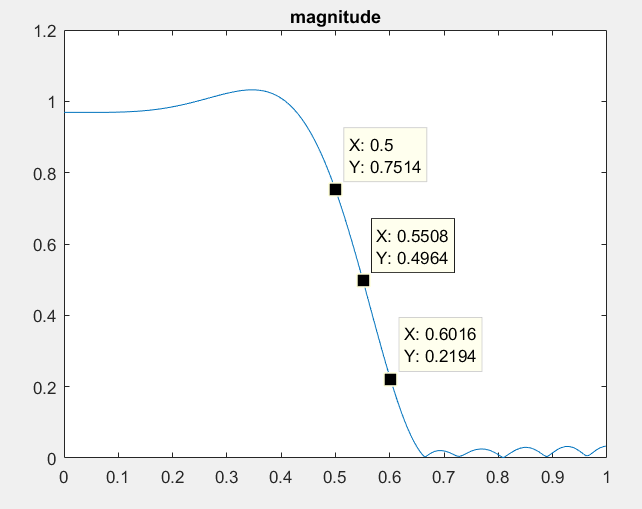
\includegraphics[width = 0.5\textwidth]{./data/solution3b.png}  
   \caption{Applying frequency transformation}
\end{figure}
\noindent \textbf {3(c)}
Using this way, we have an IIR filter with smaller ripple, and nearly equiripple.However, it has larger transitionband\\

\noindent \textbf {4(a)}
\begin{lstlisting}
b = firpm(14, [0,0.25,0.45,1], [1,1,0,0]);
[h,w]=freqz(b);
plot(w/pi,abs(h));
title('magnitude')

figure
b = firpm(14, [0,0.5,0.6,1], [0,0,1,1]);
[h,w]=freqz(b);
plot(w/pi,abs(h));
title('magnitude')
\end{lstlisting}
\begin{multicols}{2}
\begin{figure}[H]
   \centering
   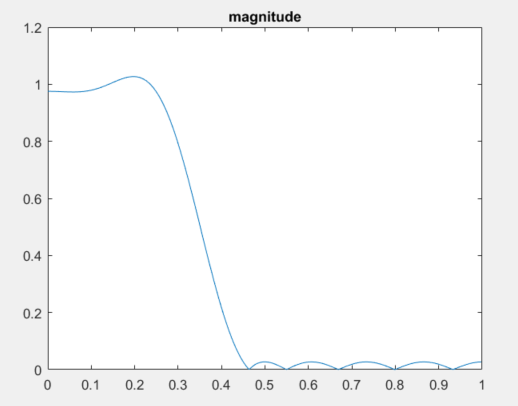
\includegraphics[width = 0.5\textwidth]{./data/solution4a1.png}  
   \caption{$\omega_c = 0.35\pi$}
\end{figure}
\begin{figure}[H]
   \centering
   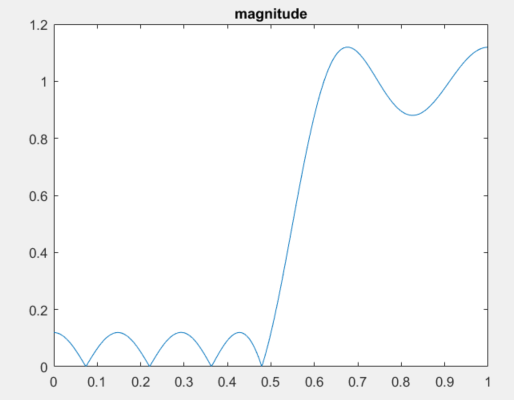
\includegraphics[width = 0.5\textwidth]{./data/solution4a2.png}  
   \caption{$\omega_c = 0.55\pi$}
\end{figure}
\end{multicols}
\noindent \textbf {4b}
\begin{lstlisting}
b = firpm(14, [0,0.25,0.45,1], [1,1,0,0]);
[h,w]=freqz(b);
plot(w/pi,abs(h));
title('magnitude')


beta = cos(0.45*pi)/cos(0.1*pi);
Mat = zeros(14,15,15);
for i = 1 : 14
    Mat(i,:,1) = [1,-beta,zeros(1,13)];
end
for i = 1 : 14
    Mat(i,:,15) = [beta,-1,zeros(1,13)];
end
for j = 2:13
    for i = 1 : j-1
        Mat(i,:,j) = [beta,-1,zeros(1,13)];
    end
    for i = j : 14
        Mat(i,:,j) = [1,-beta,zeros(1,13)];
    end
end

sum = zeros(1,15);
for l = 1 : 15
    multiTemp = ones(1,15);
    for i = 1 : 14
        multiTemp = multiTemp .* fft(Mat(i,:,l));
    end
    sum = sum + ifft(multiTemp) * b(l);
end
dedominator = zeros(1,15);
for i = 0 : 14
    dedominator(i+1) = nchoosek(14,i)*((-beta)^i);
end
figure
[h,w]=freqz(sum,dedominator);
plot(w/pi,abs(h));
title('magnitude')
\end{lstlisting}
\begin{figure}[H]
   \centering
   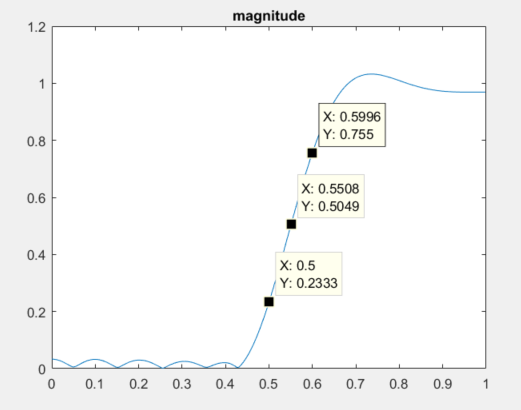
\includegraphics[width = 0.6\textwidth]{./data/solution4b.png}  
   \caption{Frequency transformation}
\end{figure}
\end{document}